\documentclass[12pt]{article}
\usepackage[shortlabels]{enumitem}
\usepackage{placeins}
\usepackage{graphicx}
\begin{document}
\title{TCSS 420 - Week 8}
\author{Jake McKenzie}
\maketitle
\noindent\centerline{\textbf{Homework 6}}
\textbf{Section 1}
8.9 Explain the difference between internal and external fragmentation.
\\\\
\textbf{Answer: }Internal fragmentation occurs when memory is divided into fixed sized partitions, by 
which a process has allocated more memory than is required, making less space available 
overall. This can be fixed by allowing variable sized partitions or by using dyanmic memory. 
\\\\
External fragmentation occurs when memory is divided into variable sized partitions, by 
which a process has allocated more memory than is required, leading to fewer and fewer 
contigious blocks of memory. This can be fixed by allowing for compaction, paging and 
segmentation.
\\\\
8.11 Given six memory partitions of $300 KB$, $600 KB$, $350 KB$, $200 KB$, $750 KB$,
and $125 KB$ (in order), how would the first-fit, best-fit, and worst-fit
algorithms place processes of size $115 KB$, $500 KB$, $358 KB$, $200 KB$, and
$375 KB$ (in order)? Rank the algorithms in terms of how efficiently they
use memory.
\\\\
\textbf{Answer: } Let $P_0$ $=$ $115$ KB, $P_1$ $=$ $500$ KB, $P_2$ $=$ $358$ KB, 
$P_3$ $=$ $200$ KB, and $P_4$ $=$ $375$ KB.
\\\\
Worst Fit $<$ First Fit $<$ Best Fit
\\
\begin{table}[htb]
\centering
\caption{First Fit}
\begin{tabular}{|c|c}
\cline{1-1}
Memory      &                               \\ \cline{1-1}
$P_0$       & 300 KB                        \\ \cline{1-1}
$P_1$       & 600 KB                        \\ \cline{1-1}
$P_3$       & 350 KB                        \\ \cline{1-1}
            & 200 KB                        \\ \cline{1-1}
$P_2$, $P_4$       & 750 KB                        \\ \cline{1-1}
            & 150 KB                        \\ \cline{1-1}
\end{tabular}
\end{table}
\\
\begin{table}[htb]
\centering
\caption{Best Fit}
\begin{tabular}{|c|c}
\cline{1-1}
Memory      &                               \\ \cline{1-1}
       & 300 KB                        \\ \cline{1-1}
$P_1$       & 600 KB                        \\ \cline{1-1}
       & 350 KB                        \\ \cline{1-1}
$P_3$            & 200 KB                        \\ \cline{1-1}
$P_2$, $P_4$       & 750 KB                        \\ \cline{1-1}
$P_0$            & 150 KB                        \\ \cline{1-1}
\end{tabular}
\end{table}
\\
\begin{table}[htb]
\centering
\caption{Worst Fit}
\begin{tabular}{|c|c}
\cline{1-1}
Memory      &                               \\ \cline{1-1}
       & 300 KB                        \\ \cline{1-1}
$P_2$       & 600 KB                        \\ \cline{1-1}
$P_3$      & 350 KB                        \\ \cline{1-1}
            & 200 KB                        \\ \cline{1-1}
$P_0$, $P_1$       & 750 KB                        \\ \cline{1-1}
            & 150 KB                        \\ \cline{1-1}
\end{tabular}
\end{table}
\FloatBarrier
\noindent 8.17 Compare paging with segmentation with respect to how much memory
the address translation structures require to convert virtual addresses to
physical addresses.
\\\\
\textbf{Answer: }Segmenation will have external fragmentation because the segments 
can be arbitrary size and may not be able to fit in empty regions of memory with no internal 
fragmentation because the size of the segment matches the size of the request. The segment table
maintains the base address the length of the segment, and segment number (index). The logical 
address a program uses is some combination of a segment number and some offset. This logical 
address is added to te base address is what a program uses to navigate memory.\\\\
In paging the logical address space can exceed currently available memory and is accomplished 
by storing portions of the unused program on disk, instead of memory. At first portions of a 
program are split up on disk, after which these portions are given specific page adresses, which 
needn't be contigious for instance for a program $\tau$ and a $\psi$ split in portions $\{\tau_0, 
\tau_1. \tau_2\}$ and $\{\psi_0, \psi_1\}$  on disk the following ordering is valid:\\
\begin{table}[htb]
\centering
\caption{Paging}
\begin{tabular}{|c|c}
\cline{1-1}
Page Address      &              Memory                 \\ \cline{1-1}
\vdots      & \vdots                        \\ \cline{1-1}
$0x8$       & $\tau_0$                        \\ \cline{1-1}
$0x9$      & $\tau_1$                        \\ \cline{1-1}
$0xA$           & $\psi_0$                        \\ \cline{1-1}
$0xB$       & $\tau_2$                        \\ \cline{1-1}
$0xC$         & $\psi_1$                        \\ \cline{1-1}
\vdots      & \vdots                        \\ \cline{1-1}
\end{tabular}
\end{table}
\FloatBarrier
\noindent In pages, each process in memor has it's own page table. Each frame memory holds exactly a flag 
for whether it is in memory or on disk in the process's table.\\\\
Paging allows you to have larger address space without more phyiscal memory, while segmentation 
does not. The programmer is not aware of pages, as it is an operaiton taken care of by the OS, while 
segmentation is visible and used by the programmer. Pages do not allow for extra security features 
while segmentation allows you to. Changing data in segmentation allows for individual compilation 
of that changed segment while paging requires a complete compile. \\\\
8.20 Assuming a 1-KB page size, what are the page numbers and offsets for
the following address references (provided as decimal numbers):\\\\
\textbf{Answer: } The logical address length is $\log_2{1024}$ $=$ $10$ and the page number is the 
rest of the bits. I like working in Hex, denoted by: page number$.$offset\\\\
a) $3085_{10}$ $=$ $0x3.0xD$ = $3_{10}.13_{10}$\\
b)  $42095_{10}$ $=$ $0x29.0x6F$ = $41_{10}.111_{10}$\\
c)  $215201_{10}$ $=$ $0xD2.0xA1$ = $210_{10}.161_{10}$\\
d)  $650000_{10}$ $=$ $0x27A.0x310$ = $634_{10}.784_{10}$\\
e)  $2000001_{10}$ $=$ $0x200.0x1$ = $512_{10}.1_{10}$\\
\\\\
\\\\8.21 a) The BTV operating system has a 21-bit virtual address, yet on certain
embedded devices, it has only a 16-bit physical address. It also has a
2-KB page size. How many entries are there in a conventional single-level page table?\\\\
\textbf{Answer: } $2^10 = 1024$
\\\\
\\\\8.22 What is the maximum amount of physical memory?\\\\
\textbf{Answer: } The maximum amount of memory in a BTV operating system is 64 KB.
\\\\
\\\\8.23 Consider a logical address space of 256 pages with a 4-KB page size,
mapped onto a physical memory of 64 frames.  How many bits are required in the logical address?
How many bits are required in the physical address?
\textbf{Answer: } $4$ KB $=$ $4$ $*$ $2^{10}$ $=$ $2^{12}$\\\\
The number of bits required for logical address is $\log_2{256} + 
\log_2{2^{12}} = \log_2{2^8} + \log_2{2^{12}} = 8 + 12 = 20$\\\\
The number of bits required for logical address is $\log_2{64} + 
\log_2{2^{12}} = \log_2{2^6} + \log_2{2^{12}} = 6 + 12 = 18$
\\\\
\\\\8.24 Consider a computer system with a 32-bit logical address and 4-KB page
size. The system supports up to 512 MB of physical memory. How many
entries are there in each of the following?\\\\
a) a conventional single-level page table: \\\\
\textbf{Answer: } Entries $=$ $\frac{logical memory space}{physical memory} 
= \frac{2^{32}}{2^{12}} = 2^{20} =$ 1MB \\\\
b) An inverted page table\\\\
\textbf{Answer: } Entries $=$ $\frac{physical memory size}{page size} = 
\frac{2^9*2^{20}}{2^2*2^{10}}=2^{17} = $ 128KB
\\\\
\\\\8.25 with TLB hitrate $= 95\%$...Consider a paging system 
with the page table stored in memory:\\\\
a) If a memory reference takes 50 nanoseconds, how long does a
paged memory reference take?\\\\
\textbf{Answer: } $4*($Time to access page table $\times$ Time to access word in memory$) = 
4*(50$ns $+$ $50$ns$) = 4*10$ns$400$ns\\\\
b) If we add TLBs, and 75 percent of all page-table references are found
in the TLBs, what is the effective memory reference time? (Assume
that finding a page-table entry in the TLBs takes 2 nanoseconds, if
the entry is present.)\\\\
\textbf{Answer: } $0.95*200+0.05*400=210$ns
\\\\
\\\\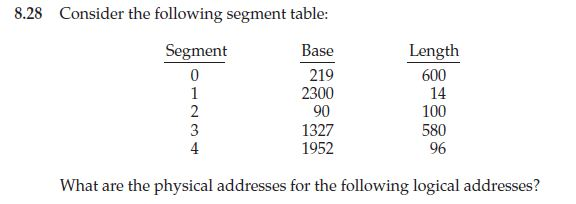
\includegraphics[scale = 1]{28.jpg}\\
\textbf{Answer: } a) $219+430=649$\\
b) $2300+10=2310$\\
c) Trap thrown by OS\\
d) $1327+400=1727$\\
e) Trap thrown by OS
\\\\
\\\\8.29 What is the purpose of paging the page tables?\\\\
\textbf{Answer: }Firstly it puts the user page tables in a pageable segment of 
the system's address space. Seconly it allows the system segment containing the user page 
tables to be paged. Lastly it allws you to reduce the physical memory requirements of page 
tables by mapping a portion of the address space to that is actually being used.
\\\\
\\\\8.32 Consider the Intel address-translation scheme shown in Figure 8.22.\\\\
a) Describe all the steps taken by the Intel Pentium in translating a
logical address into a physical address.\\\\
\textbf{Answer: } The selector is an index into the segment descriptor table. 
The segment descriptor result plus the original offset is used to produce a linear 
address with dir$\rightarrow$page$\rightarrow$offset. The dir is an index into a page directory; 
the entry from this directory selects the page table, 
and the page field is an index into that page table. The entry from the page 
table, plus the offset, is the physical address.
\\\\
b) What are the advantages to the operating system of hardware that
provides such complicated memory translation?\\\\
\textbf{Answer: }This allows for a level of abstraction that allows for 
various hardware configurations. Because it allows for different hardware configurations 
it allows for more efficiencies.
c) Are there any disadvantages to this address-translation system? If
so, what are they? If not, why is this scheme not used by every
manufacturer?\\\\
The restriction here is on how long it takes for table lookup, which while be $O(1)$ time 
runtime in reality can add up if not taken into account. Caches can help, but you can still 
have a cache miss.
\\\\ \textbf{Section 2}
\\\\
\\\\a)
\textbf{Answer: }
\\\\
\\\\b)
\textbf{Answer: }
\\\\ \textbf{Section 3}
\textbf{Answer: }
\\\\
\\\\ \textbf{Section 4}
\textbf{Answer: }
\\\\
\end{document}